\chapter{Processo de Engenharia de Requisitos}

  Neste tópico será apresentado o processo de Engenharia de Requisitos elaborado para o projeto, descrevendo quais os papeis,
  atividades e artefatos que serão utilizados no mesmo, e sua respectiva modelagem criada na ferramenta draw.io, que é uma
  ferramenta online de desenhos UML e de modelagem.

  A abordagem utilizada foi a abordagem ágil, fundamentada no \textbf{SAFe} (Scaled Agile Framework), que permite escalar práticas
  ágeis em organizações e projetos, provendo artefatos, papéis e atividades em três níveis estruturais do framework: \textbf{Portfolio},
  que é o nível mais alto da abstração, levantados os requisitos de mais alto nível, sendo eles os temas de investimentos, épicos e
  épicos enables, \textbf{Programa}, que é o nível que faz a comunicação entre o portifolio e o time, neste nível os requisitos
  levantados no portifolio são transformados em features e os program increments são planejados e o ultimo é o nível de \textbf{Time},
  que é o nível mais baixo utilizando o SCRUM, as features são quebradas em histórias de usuários e são implementadas e todos os
  eventos do scrum estão presentes nesse nível. O nível de \textbf{Fluxo de Valor presente} na versão 4.0 do SAFe não será utilizado,
  pois não há necessidade deste nível nesse projeto.

  A estrutura dos três níves do SAFe foi mantida porque, segunda Leffingwell (2011), ao diminuir o nível de abstração dos requisitos
  gradativamente, reduz também o nível de especificação precoce, diminuindo a sobrecarga ao gerenciar os requisitos. Isso também
  aumenta a agilidade do time por permitir a interpretação dos requisitos de maneira mais fácil para a implementação.

  Logo abaixo será especificado como tratam sobre o modelo do processo de Engenharia de Requisitos, apelidado de \textbf{Big Picture}
  do projeto, os papéis desempenhados e as atividades e artefatos envolvidos no processo.

\section{Modelo de Processo de Engenharia de Requisitos}

  \begin{figure}[!htb]
    \centering
    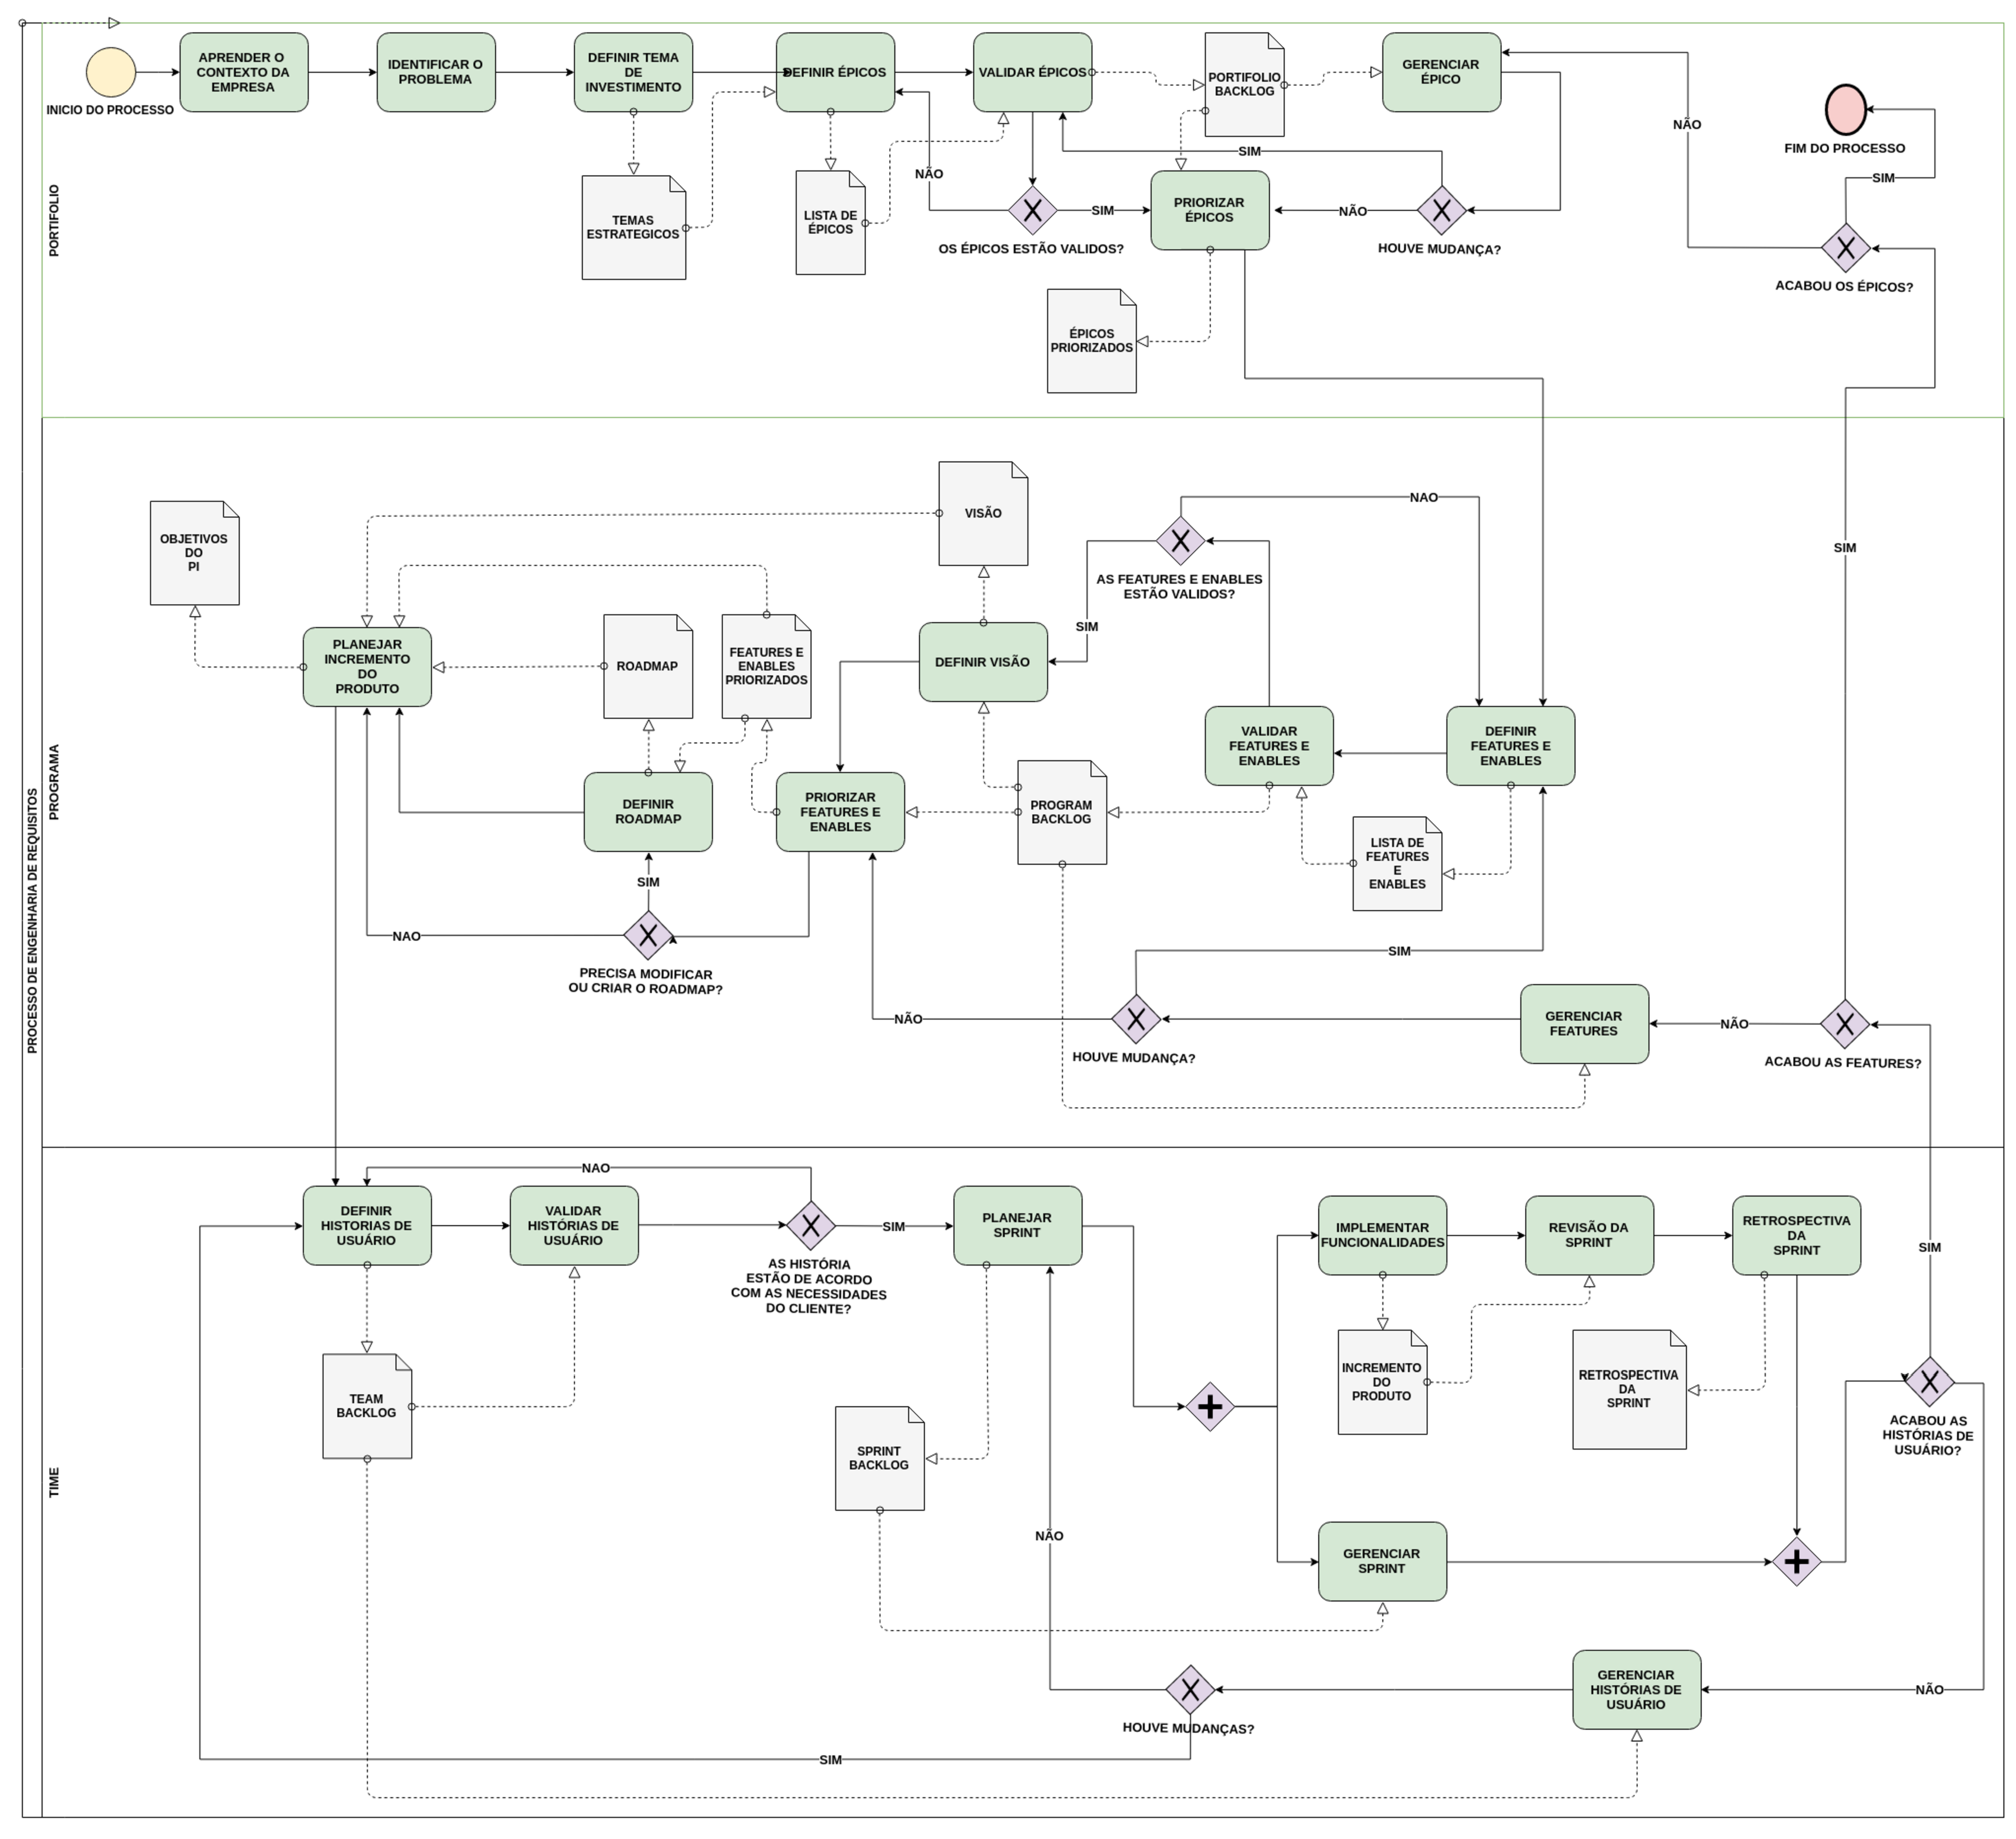
\includegraphics[width=17cm, keepaspectratio=true]{figuras/maturidade/processo.eps}
    \caption{Processo da Engenharia de Requisitos}
  \end{figure}

  \newpage

\section{Papéis}

\subsection{\textbf{Portfólio}}

  \begin{itemize}
    \item \textbf{Gerente de Portfólio de Programa}: Representa a pessoa que tem mais impacto nas decisões tantos estratégicas quanto
      financeiras dentro do framework, e entende os limites da estratégia de negócio da empresa, de tecnologia e de fundos. Uma de suas
      responsabilidades é de participar das sessões de escolha e comunicação dos temas de investimento e da definição e priorização do
      backlog de épicos.
    \item \textbf{Gerente de Épicos}: Representa o papel na qual toma-se a responsabilidade de gerenciar épicos individuais por todo o
      processo de portifolio kanban, desenvolvendo casos de negócios. Trabalha-se com os principais stakeholders na análise de valor
      agregado do épico. Quando o épico é aprovado, o gerente de épico trabalha com o time de desenvolvimento e o gerente de produto
      para estabelecer as atividades de desenvolvimento, para que as mesmas atinjam os benefícios de negócios do épico em especifico.
    \item \textbf{Arquiteto da empresa}: Representa a pessoa que sempre visa manter uma visão geral das tecnologias, soluções da
      empresa e iniciativas de desenvolvimento. Uma de suas atividades é entender e comunicar os temas de investimento e outras chaves
      de negócios para os arquitetos de sistema e stakeholders não técnicos, e também influenciar na decisão de uma modelagem comum e
      em boas práticas de codificação.
  \end{itemize}

\subsection{\textbf{Programa}}

  \begin{itemize}
    \item \textbf{Gerente de Releases}: Representa a pessoa que planeja a release, e coordena a implementação de todas as capacidades e
      funcionalidades nas diversas iterações dentro de uma release. Um de seus papéis é comunicar o status da release para stakeholders
      externos a empresa, e também de prover uma autorização final da release.
    \item \textbf{Gerente de Produto}: Junto do Gerente de Soluções, eles formam as principais autoridades de conteúdo. Eles criam a
      visão do programa, trabalham com os clientes e também com os Product Owners para entenderem e comunicarem as necessidades,
      participam na validação de soluções propostas, define os requisitos, gerencia e prioriza o fluxo de trabalho e também define
      releases e Program Increments.
  \end{itemize}

\subsection{\textbf{Time}}

  \begin{itemize}
    \item \textbf{Product Owner (P.O)}: Representa a pessoa que tem como responsabilidade a definição das histórias de usuário e de
      priorizar o backlog de time. O P.O desempenha um papel importantíssimo no quesito qualidade, pois é o único do time que tem a
      responsabilidade de aceitar as histórias como finalizadas. É bastante envolvido na construção do backlog do programa e na
      preparação e refinamento do planejamento do PI
    \item \textbf{Scrum Master}: Representa a pessoa que está sempre monitorando a equipe com o intuito de fazer com que todos sigam
      a metodologia, ou seja, o Scrum Master monitora os integrantes para que todos cumpram e sigam os princípios da metodologia.
      Uma das responsabilidades do Scrum Master é manter a equipe focada nos objetivos certos, assegurando um fluxo de produtividade
      o mais alto possível. Também tem como responsabilidade facilitar os encontros do time, tanto no planejamento quanto na
      retrospectiva e revisão da sprint.
    \item \textbf{Desenvolvedores}: Representa as pessoas que vão de fato construir o sistema, produzindo o código fonte e os testes
      da aplicação. Participa de todas as atividades do processo no nível de time.
    \item \textbf{Equipe}: Representa a junção dos três citados acima.
  \end{itemize}

\section{Descrição das atividades}

\subsection{\textbf{Portfólio}}

\subsubsection{Aprender contexto da empresa}

  \begin{itemize}
    \item \textbf{Entrada:} Contexto da empresa.
    \item \textbf{Saída:} Entendimento das políticas e negócios da empresa.
    \item \textbf{Responsável:} Time.
    \item A primeira atividade do processo é aprender o contexto da empresa, suas políticas e negócios, através de encontros com o
      cliente, buscando um primeiro contato e estabelecendo um canal de comunicação com o cliente.
  \end{itemize}

\subsubsection{Identificar o problema}
  \begin{itemize}
    \item \textbf{Entrada:} Contexto da empresa.
    \item \textbf{Saída:} Visão geral das necessidades da empresa.
    \item \textbf{Responsável:} Gerente de portfólio.
    \item Essa atividade visa fazer reuniões com o product owner, utilizando as tecnicas de elicitação de requisitos para levantar os
      possiveis problemas.
  \end{itemize}

\subsubsection{Definir temas de investimento}
  \begin{itemize}
    \item \textbf{Entrada:} Problema identificado.
    \item \textbf{Saída:} Temas de investimento.
    \item \textbf{Responsável:} Gerente de portfólio.
    \item Essa atividade é responsável por gerar e documentar os temas de investimento, a partir do contexto da empresa e os problemas.
      Esses temas de investimentos serão levantados com o product owner, utilizando as técnicas de elicitação.
  \end{itemize}

\subsubsection{Definir Épicos}
  \begin{itemize}
    \item \textbf{Entrada:} Temas de investimento.
    \item \textbf{Saída:} Lista de épicos.
    \item \textbf{Responsável:} Gerente de portifolio.
    \item Essa atividade é responsável por englobar todos os épicos propostos, tanto épicos de negocio como épicos de enable, em uma fase
      inicial, na qual nem todos os épicos que foram propostos irão ser definidos.
    \item A partir dos épicos propostos, é definido o backlog de épicos para a realização do tema de investimento, tendo também os épicos
      enables, que são os itens de trabalho necessários para apoiar   a implementação dos Épicos, também conhecidos como requisitos não
      funcionais.
  \end{itemize}

\subsubsection{Validar Épicos}
  \begin{itemize}
    \item \textbf{Entrada:} Lista épicos.
    \item \textbf{Saída:} Portfólio backlog.
    \item \textbf{Responsável:} Gerente de épicos.
    \item Com a lista de épicos feito, é realizado uma validação deles com o cliente, para confirmar que é esse o produto que eles
      tinham em mente.
  \end{itemize}

\subsubsection{Priorizar Épico}
  \begin{itemize}
    \item \textbf{Entrada:} Portfolio de épicos.
    \item \textbf{Saída:} Épicos priorizados.
    \item \textbf{Responsável:} Gerente de épicos.
    \item Dado o Portifolio de épicos concluído e validado, juntamente com o cliente é escolhido o mais importante dentro dos que
      ainda não foram implementados.
  \end{itemize}

\subsubsection{Gerenciar Épicos}
  \begin{itemize}
    \item \textbf{Entrada:} Portifolio de épicos.
    \item \textbf{Responsável:} Gerente de portifolio.
    \item O gerente de portfolio junto ao resto da equipe irão verificar se existem mais épicos no portfolio backlog ou se é
      necessária a criação de novos épicos.
  \end{itemize}

\subsection{\textbf{Programa}}

\subsubsection{Definir features e enables}
  \begin{itemize}
    \item \textbf{Entrada:} Épicos priorizados.
    \item \textbf{Saída:} Lista de features e enables.
    \item \textbf{Responsável:} Gerente de produto.
    \item A partir da realização de reuniões com o cliente, utilizando as tecnicas de elicitação, serão levantados algumas condições
      para a construção da solução, sendo algumas dessas condições ferramentas que irão auxiliar na implementação dessas
      funcionalidades como padrões de projeto, arquitetura, servidores, acessibilidade, etc (requisitos não funcionais ou enables)
      e outras funcionalidades do produto (requisitos funcionais ou features), na qual nem todos os requisitos que foram propostos
      irão ser definidos.
  \end{itemize}

\subsubsection{Validar Features e enables}
  \begin{itemize}
    \item \textbf{Entrada:} Lista de Features e enables definidas.
    \item \textbf{Saída:} Definição do documento de visão e do program backlog.
    \item \textbf{Responsável:} Gerente de produto
    \item Com as features e enables definidas, cada uma deve receber uma pontuação de acordo com sua relev\^{a}ncia, ou seja, valor
      que agrega para o cliente e dificuldade de implementação.
  \end{itemize}

\subsubsection{Definir Visão}
  \begin{itemize}
    \item \textbf{Entrada:} Program backlog com os requisitos validados.
    \item \textbf{Saída:} Documento de Visão do produto.
    \item \textbf{Responsável:} Gerente de produto.
    \item Com os requisitos validados a equipe terá uma noção de como vai funcionar o produto, ter uma visão geral dele.
  \end{itemize}

\subsubsection{Priorizar Features e enables}
  \begin{itemize}
    \item \textbf{Entrada:} program backlog.
    \item \textbf{Saída:} Features e enables priorizados para incremento.
    \item \textbf{Responsável:} Gerente de produto
    \item Com as features e enables validadas, o gerente de produto ira definir quais features e anables irá para o incremento do produto
  \end{itemize}

\subsubsection{Definir Roadmap}
  \begin{itemize}
    \item \textbf{Entrada:} Program backlog com os requisitos validados e priorizados.
    \item \textbf{Saída:} Roadmap: Planejamento do incremento do produto.
    \item \textbf{Responsável:} Gerente de release.
    \item Com as features e enables validados e priorizados a equipe terá uma noção do planejamento das séries de releases, cada uma
      pertinente a um tema, um conjunto de objetivos e a priorização das features. O Roadmap nos dá uma ideia de como a equipe
      planeja mostrar valor no decorrer do tempo.
  \end{itemize}

\subsubsection{Planejar Incremento do Produto}
  \begin{itemize}
    \item \textbf{Entrada:} Definição do roadmap, da visão e o program backlog com os requisitos validados e priorizados.
    \item \textbf{Saída:} Objetivos da PI
    \item \textbf{Responsável:} Gerente de produto.
    \item Através da visão do produto com suas features e enables e do roadmap com o planejamento de todas as releases do produto,
      além dos requisitos validados e priorizados para a sprint que será planejada, o planejamento do incremento do produto tem como
      artefato o objetivos do PI, que é a conexão do time de desenvolvimento com a equipe de negócios da empresa/cliente em relação
      as features que vai ser implementada nesse incremento do produto ou sprint.
  \end{itemize}

\subsubsection{Gerenciar Features}
  \begin{itemize}
    \item \textbf{Entrada:} Program backlog.
    \item \textbf{Responsável:} Gerente de release.
    \item O gerente de release junto ao resto da equipe irão verificar se existem mais features ou enables no program backlog ou se é
      necessária a criação de novas features ou enables.
  \end{itemize}

\subsection{\textbf{Time}}

\subsubsection{Definir Histórias de Usuário}
  \begin{itemize}
    \item \textbf{Entrada} Features e enables planejadas para o incremento
    \item \textbf{Saída:} Team backlog
    \item \textbf{Responsável:} Equipe
    \item Através dos Planejamento do incremento do produto, na qual vai incluir as features e enables que forám priorizados para esse
      incremento, será criado o Team backlog com todas as histórias de usuário para validação
  \end{itemize}

\subsubsection{Validar Histórias de Usuário}
  \begin{itemize}
    \item \textbf{Entrada:} Team backlog
    \item \textbf{Saída:} Team backlog validada
    \item \textbf{Responsável:} Equipe
    \item Junto com o product owner e o scrum master a equipe irá validar todas as histórias que irão agregar valor ao produto e ao
      cliente para serem implementadas.
  \end{itemize}

\subsubsection{Planejar a Sprint}
  \begin{itemize}
    \item \textbf{Entrada:} Team backlog valido.
    \item \textbf{Saída:} Backlog da sprint.
    \item \textbf{Responsável:} Equipe
    \item Através do team backlog validado, iremos criar o backlog da sprint com as historias de usuário que iremos implementar nesse
      incremento do produto através de iterações.
  \end{itemize}

\subsubsection{Implementar Funcionalidades}
  \begin{itemize}
    \item \textbf{Entrada:} Sprint planejada com o backlog da sprint.
    \item \textbf{Saída:} Incremento do produto
    \item \textbf{Responsável:} desenvolvedores
    \item A equipe de desenvolvimento irá com as história de usuário planejadas para aquelas sprint, criar um incremento do produto
      para entregar ao cliente.
  \end{itemize}

\subsubsection{Realizar Revisão da Sprint}
  \begin{itemize}
    \item \textbf{Entrada:} Histórias das sprints implementadas.
    \item \textbf{Saída:} Revisão completa das novas funcionalidades.
    \item \textbf{Responsável:} Equipe
    \item A equipe irá fazer uma revisão completa das novas funcionalidade implementadas no produto
  \end{itemize}

\subsubsection{Realizar Retrospectiva da Sprint}
  \begin{itemize}
    \item \textbf{Entrada:} Revisão da sprint efetuada.
    \item \textbf{Saída:} Verificar se existem mais features e quais foram os pontos positivos e negativos da sprint
    \item \textbf{Responsável:} Equipe
    \item A equipe irá fazer uma retrospectiva para ver se existem mais features e quais foram os pontos positivos e negativos da
      sprint para poder melhorar nas próximas.
  \end{itemize}

\subsubsection{Gerenciar sprint}
  \begin{itemize}
    \item \textbf{Entrada:} sprint backlog.
    \item \textbf{Responsável:} product owner.
    \item O product owner junto ao resto da equipe irão verificar se existem mais histórias de usuário na sprint backlog para ser
      implementadas.
  \end{itemize}

\subsubsection{Gerenciar História de Usuário}
  \begin{itemize}
    \item \textbf{Entrada:} team backlog.
    \item \textbf{Responsável:} product owner.
    \item O product owner junto ao resto da equipe irão verificar se existem mais histórias de usuário na team backlog para ser
      inserida no planejamento das sprints ou se é necessária a criação de novas histórias.
  \end{itemize}

\section{Maturidade}

\subsection{CMMI (Capability Maturity Model $-$ Integration)}

  O CMMI é um modelo de maturidade internacional, geralmente utilizado por empresas
  globalizadas que necessitam de certificação para serem reconhecidos internacionalmente.
  Surgiu como integração e evolução dos modelos SW-CMM (Capability Maturity Model for Software),
  SECM EIA 731 (System Engineering Capability Model) e  e IPD-CMM
  (Integrated Product Development CMM).\cite{mct2006}.

  O CMMI possui 5 níveis de maturidade, enumerdos do 1 ao 5 e cada nível corresponde
  à capacidade da organização de desenvolvimento do produto, sendo o nível 1 o mais
  baixo nível de maturidade e o nível 5 o mais alto e contínuo.

  \begin{figure}[!ht]
    \centering
    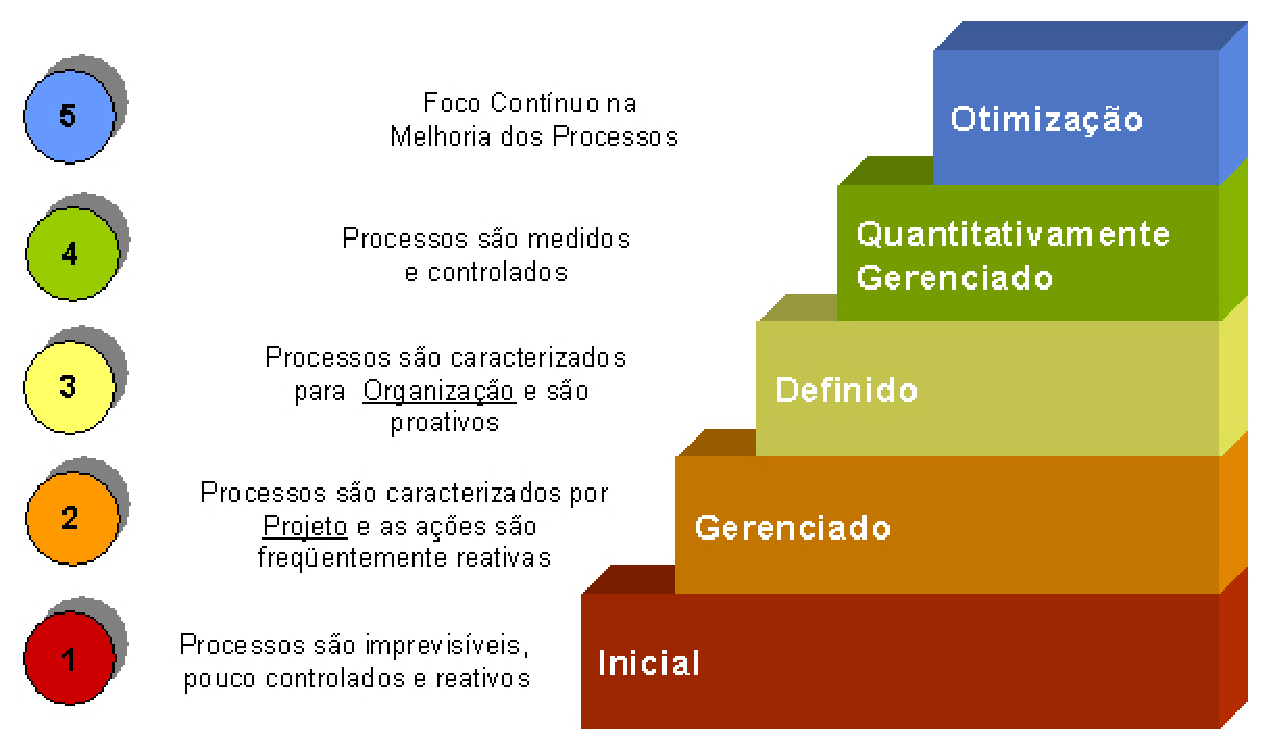
\includegraphics[width=15cm, keepaspectratio=true]{figuras/maturidade/niveis-cmmi.eps}
    \caption{Os cinco níveis de maturidade do modelo CMMI}
  \end{figure}

\subsubsection{Vantagens}

  Como já dito na descrição na Subseção 1.1, o CMMI é um modelo de melhoria
  de processos reconhecido internacionalmente, fazendo com que a organização
  certificada por ele tenha a vantagem de ser reconhecida em qualquer lugar
  do mundo por causa da aplicação do CMMI

  Com o CMMI, a organização vai se otimizando cada vez mais e o controle do
  processo fica cada vez mais definido, sendo assim, a organização continuamente
  vai identificando o que realmente tem valor de acordo com sua maturidade.

\subsubsection{Desvantagens}

  O CMMI tem um alto custo, por isso geralmente quem tem a certificação são
  grandes organizações globalizadas que possuem recursos para sustentar a
  avaliação e se torna vantajoso para seu reconhecimento internacional. O
  tempo para amadurecimento do processo pode levar de 4 a 8 anos, sendo assim
  definido um modelo moroso e caro. Segundo Franciscani, algumas organizações
  tratam o CMMi como um processo e não como modelo, fazendo com que eles tenham
  a percepção de que nem tudo que está no CMMI seja mesmo necesário.\cite{francis2012}.

\subsection{MPS.BR}

  O modelo MPS.BR foi desenvolvido pela Softex com o objetivo de atingir
  certificações de pequenas e médias empresas, bem como possibilitar que
  as empresas possam ter acesso mais facilitado para a certificação.
  O modelo MPS.BR se adequa ao mercado brasileiro de software e deriva do CMMI
  Enquanto o CMMI possui cinco níveis de maturidade enumeradas do 1 ao 5, o
  MPS.BR possui sete níveis classificados, de forma piramidal,  pelas letras
  do A ao G, sendo o nível A o mais alto e contínuo nível de maturidade e o G
  o mais baixo. A Figura 2 contém a representação dos níveis de maturidade do
  MPS.BR

  \begin{figure}[!ht]
    \centering
    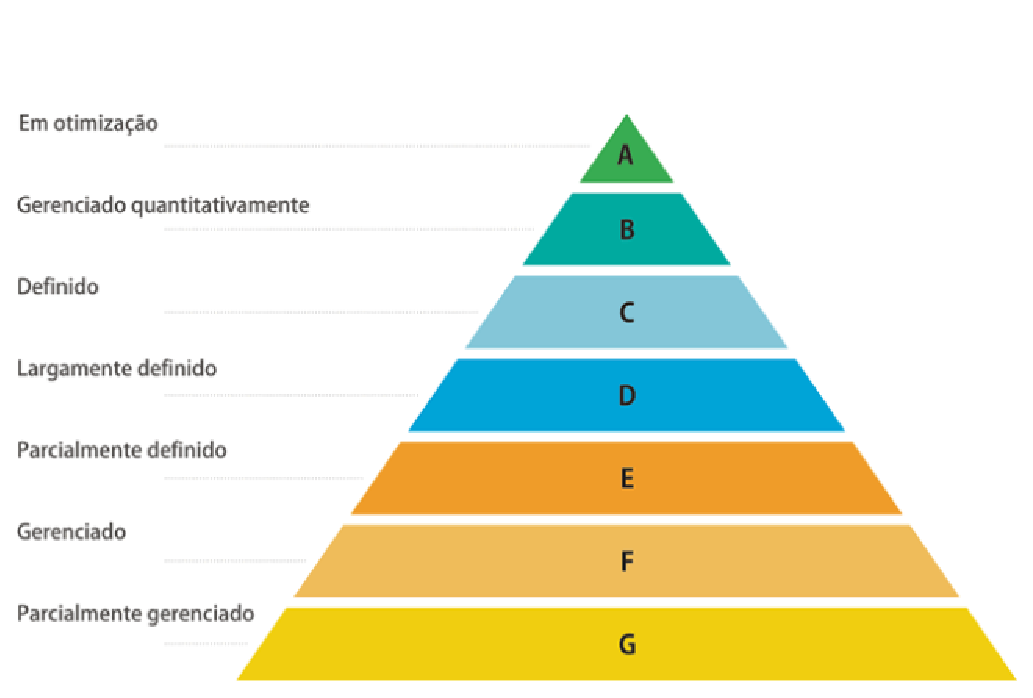
\includegraphics[width=15cm, keepaspectratio=true]{figuras/maturidade/niveis-mpsbr.eps}
    \caption{Os sete níveis de maturidade do modelo MPS.Br}
  \end{figure}

\subsubsection{Vantagens}

  Além do MPS.BR ser mais acessível e estar mais adequado ao contexto de
  organizações brasileiras, segundo Franciscani, existem outras vantagens
  como:

  \begin{itemize}
    \item{Compatibilidade com CMMI, podendo ser aproveitado para uma futura
          certificação nesse modelo.}
    \item{Dois números de nível a mais do que do CMMI, o que pode facilitar a
          implantação em pequenas e médias organizações.}
    \item{Obrigatoriedade do certificado em licitações.}
    \item{Integração Universidade-Empresa.}
  \end{itemize}

\subsubsection{Desvantagens}

  O MPS.BR não possibilita as empresas serem competitivas internacionalmente,
  por ser um modelo que se adequa apenas para certificação nacional. Isso pode
  ser uma desvantagem muito grande para organizações que pretendem
  globalizar-se.\cite{francis2012}.

\subsection{Seleção do Modelo}

  A Cráton é uma empresa júnior com apenas 15 membros formada por estudantes no qual
  não visam lucro para si mesmos, pois todo o dinheiro obtido deve ser investido
  na própria empresa como consta na lei número 13.267 de 2016 que regulamenta as empresas
  juniores e as define com fim educacional e não lucrativo. Neste contexto, o CMMI seria
  impraticável devido ao alto custo e a limitação de crescimento de uma empresa júnior que é
  completamente dependente das universidades e não seria globalizada, não precisando do CMMI

  O grupo possui quatro integrantes, o que se encaixa no contexto do MPS.BR que se direciona
  principalmente para organizações menores, fazendo-se ser mais acessível para poder desenvolver
  o modelo dentro do contexto do cliente.

  O cliente, sendo uma empresa júnior integrada com a Universidade de Brasília, poderia se
  beneficiar dos processos do MPS.BR, já que é um modelo que possui integração universidade-empresa.
  Dessa forma, o modelo seria aplicado diretamente no meio acadêmico.

  Por esses motivos apontados, o modelo MPS.BR foi selecionado para a engenharia de requisitos da
  solução do problema da Cráton.

\subsection{Processos Selecionados}

  Para o contexto da disciplina, serão implementados dois processos que tratam de
  requisitos, sendo o processo de Gerência de Requisitos que se encontra no nível
  G do MPS.BR e o Desenvolvimento de Requisitos que é um processo do nível D. Nos
  subtópicos seguintes, 1.4.1 e 1.4.2, estará o propósito e os resultados esperados
  de cada processo referenciado diretamente do Guia Geral do MPS.BR.\cite{softexmps}.

\subsubsection{Gerência de Requisitos $-$ GRE}

  \begin{description}
    \item[Propósito] \
      O propósito do processo Gerência de Requisitos é gerenciar os requisitos do
      produto e dos componentes do produto do projeto e identificar inconsistências
      entre os requisitos, os planos do projeto e os produtos de trabalho do projeto.
    \item [Resultados Esperados] \
      \begin{itemize}
        \item GRE 1. O entendimento dos requisitos é obtido junto aos fornecedores de requisitos;
        \item GRE 2. Os requisitos são avaliados com base em critérios objetivos e um comprometimento
              da equipe técnica com estes requisitos é obtido;
        \item GRE 3. A rastreabilidade bidirecional entre os requisitos e os produtos de trabalho
              é estabelecida e mantida;
        \item GRE 4. Revisões em planos e produtos de trabalho do projeto são realizadas;
              visando identificar e corrigir inconsistências em relação aos requisitos;
        \item GRE 5. Mudanças nos requisitos são gerenciadas ao longo do projeto.
      \end{itemize}
    \end{description}

\subsubsection{Desenvolvimento de Requisitos $-$ DRE}

  \begin{description}
    \item [Propósito] \
     O propósito do processo Desenvolvimento de Requisitos é definir os requisitos
     do cliente, do produto e dos componentes do produto.
    \item [Resultados Esperados]\
      \begin{itemize}
        \item DRE 1. As necessidades, expectativas e restrições do cliente, tanto do produto
              quanto de suas interfaces, são identificadas;
        \item DRE 2. Um conjunto definido de requisitos do cliente é especificado e priorizado
              a partir das necessidades, expectativas e restrições identificadas;
        \item DRE 3. Um conjunto de requisitos funcionais e não-funcionais, do produto e dos componentes
                    do produto que descrevem a solução do problema a ser resolvido, é definido e mantido
                    a partir dos requisitos do cliente;
        \item DRE 4. Os requisitos funcionais e não-funcionais de cada componente do produto são
              refinados, elaborados e alocados;
        \item DRE 5. Interfaces internas e externas do produto e de cada componente do produto são
              definidas;
        \item DRE 6. Conceitos operacionais e cenários são desenvolvidos;
        \item DRE 7. Os requisitos são analisados, usando critérios definidos, para balancear
              as necessidades dos interessados com as restrições existentes;
        \item DRE 8. Os requisitos são validados.
      \end{itemize}
  \end{description}

